% Esta es la Plantilla UNAL en LaTeX
\documentclass[12pt,spanish,fleqn,openany,twoside,letterpaper]{book}

%Muestra los márgenes del documento para evitar Warnings
%Para activar la siguiente línea quite el simbolo % 
%\usepackage[showframe]{geometry}

%Formato de fuentes bibliográficas
%Use el estilo bibliográfico que sea pertinente según el área de estudio APA, IEEE, etc

%Usando el paquete BibLaTeX
%Cita normal con \cite[página]{} y cita con paréntesis \parencite[página]{}

%\usepackage[style=numeric]{biblatex}
%\addbibresource{Referencias.bib}

% Configuración de BibLaTeX
%\usepackage[backend=biber,style=authoryear,maxcitenames=2,maxbibnames=99,giveninits=true,uniquename=false]{biblatex}
%\addbibresource{biblio.bib}

% Cambiar el idioma de las referencias bibliográficas a español
%\DefineBibliographyStrings{spanish}{%
%  andothers = {et\addabbrvspace al\adddot},
%  andmore = {et\addabbrvspace al\adddot},
%}

% Personalizar el formato de las citas y la bibliografía
%\DeclareNameAlias{sortname}{family-given}
%\DeclareDelimFormat{multinamedelim}{\addcomma\space}
%\DeclareDelimFormat{finalnamedelim}{\addcomma\space\&\space}
%\DeclareFieldFormat{titlecase}{\MakeSentenceCase*{#1}}
%\DeclareFieldFormat[article,inbook,incollection,inproceedings,patent,thesis,unpublished]{title}{\titlecase{#1}}
%\DeclareFieldFormat{journaltitlecase}{\titlecase{#1}}
%\DeclareFieldFormat{pages}{#1}
%\DeclareFieldFormat{volume}{\mkbibbold{#1}}
%\renewbibmacro{in:}{}
%\AtEveryBibitem{\clearfield{month}}

%Usando el paquete Natbib
%Cita normal \cite[página]{} y cita con paréntesis \citep[página]{}
\usepackage{natbib}
\bibpunct{[}{]}{;}{\&}{.}{}
\bibliographystyle{dtvstyle}

%Idioma del documento
%Use main para el idioma principal del documento
\usepackage[main = spanish, english, german, french, portuguese]{babel}

% Carácteres especiales
\usepackage[T1]{fontenc}

%Resaltado en amarillo
\usepackage{soul}

% Evita ligadura li & fl
\usepackage{microtype}
%\DisableLigatures{encoding = *, family = *}

%Varias columnas
\usepackage{multicol}

% Otros paquetes de tablas y colores avanzados
\usepackage{amsmath,graphicx,rotating,float,multirow}
\usepackage{siunitx}
\usepackage{longtable}
\setlength{\LTcapwidth}{6in}
\usepackage[utf8]{inputenc}
\usepackage{epsfig,epic,eepic,threeparttable,amscd,here,lscape,tabularx,subfigure}
\usepackage{tabu,array}
\usepackage[rgb]{xcolor}

% Permite ver y configurar los parámetros de la página
\usepackage{layout}
%Hyperref permite ver las secciones del texto
\usepackage[hidelinks]{hyperref}

\usepackage{ragged2e}


\usepackage{comment}

%Permite incluir código de cualquier lenguaje dentro del texto del documento
\usepackage{minted}
\usepackage{fancyvrb}
\newenvironment{myverbatim}{\Verbatim}{\endVerbatim}

%Genera los comandos de la página de autoría
\newcommand{\studentname}{}
\newcommand{\submissiondate}{}
\newcommand{\academictitle}{}
\newcommand{\resgroupone}{}
\newcommand{\resgrouptwo}{}
\newcommand{\researchtopic}{}
\newcommand{\thesisname}{}
\newcommand{\thesisnameeng}{}
\newcommand{\thesisnamelang}{} %Usar solo si se requiere
\newcommand{\director}{}
\newcommand{\directortitle}{}
\newcommand{\codirector}{} %Usar solo si se requiere
\newcommand{\codirectortitle}{} %Usar solo si se requiere
\newcommand{\issuedate}{}
\newcommand{\palabrasclave}{}
\newcommand{\keywords}{}
\newcommand{\schlusselworter}{}
\newcommand{\palavraschave}{}
\newcommand{\sede}{}
\newcommand{\department}{}
\newcommand{\departmenttwo}{} %Usar solo si se requiere
\newcommand{\faculty}{}
\newcommand{\university}{Universidad Nacional de Colombia}

%Información de la tesis
%Diligenciar aquí los datos para su carga automática donde se requiera en el documento
%En el caso de tesis o trabajos finales, verificar que el título coincida con el aprobado por la Facultad
\renewcommand{\studentname}{Nombre del estudiante}
\renewcommand{\thesisname}{\nombreTesis}
\renewcommand{\thesisnameeng}{Nombre del trabajo o tesis en inglés}
\renewcommand{\thesisnamelang}{Nombre del trabajo o tesis en un tercer idioma} %Usar solo si se requiere
\renewcommand{\issuedate}{Año entrega}
\renewcommand{\submissiondate}{Fecha entrega}
\renewcommand{\director}{Prof. Dr. Director}
\renewcommand{\directortitle}{Indicar si es Profesor Titular/Asociado}
\renewcommand{\codirector}{Prof. Dr. Co director}
\renewcommand{\codirectortitle}{Indicar si es Profesor Titular/Asociado}
\renewcommand{\academictitle}{Magíster (M, MSc) o Doctor (PhD) - Modalidad }
\renewcommand{\resgroupone}{Grupo A (Sigla Grupo Investigación 01) }
\renewcommand{\resgrouptwo}{Grupo B (Sigla Grupo Investigación 02) }
\renewcommand{\researchtopic}{Línea}
\renewcommand{\sede}{Sede de la Universidad} 
\renewcommand{\department}{Departamento}
\renewcommand{\departmenttwo}{Departamento 2} %Usar solo si es necesario
\renewcommand{\faculty}{Facultad}

%Palabras clave del documento - Tener presente los Theasurus https://www.thesaurus.com/
%Disponible en 3 idiomas aunque se puede extender a francés o otro idioma
\renewcommand{\palabrasclave}{Use palabras clave que estén en Theasaurus} 
\renewcommand{\keywords}{Use keywords available in Theasaurus}
%\renewcommand{\schlusselworter}{}
%\renewcommand{\palavraschave}{}

% Estilo de los encabezados y pies de página
\usepackage{fancyhdr}
\fancyhf{}%
\pagestyle{fancyplain}
\textheight22.5cm \topmargin0cm \textwidth16.5cm \headheight22pt
\oddsidemargin0.5cm \evensidemargin-0.5cm%
\fancypagestyle{plain}{
\fancyhead[RO,LE]{}
\fancyhead[RE,LO]{\small \textbf{\thesisname}}
\fancyfoot[CO,CE]{\thepage}
}
\pagestyle{fancy}
\fancyhf{}%
\renewcommand{\chaptermark}[1]{\markboth{\thechapter.\; #1}{}}
\renewcommand{\sectionmark}[1]{\markright{\thesection.\; #1}{}}
\fancyhead[LO,RE]{\leftmark}
\fancyhead[RO,LE]{\rightmark}
\fancyfoot[CO,CE]{\thepage}
\thispagestyle{fancy}%

\usepackage{titlesec}
% Permite personalizar los títulos de sección y de capítulos
% hang lo deja en el mismo renglón, display lo despliega
% Elimina el "Capitulo" y deja solo el número
\titleformat{\chapter}[hang]
  {\sffamily\Huge\bfseries}{\thechapter}{0.5cm}{\sffamily\Huge}
\titleformat{\section}[hang]{\sffamily\LARGE}{\thesection}{0.5cm}{}
\titleformat{\subsection}[hang]{\sffamily\Large}{\thesubsection}{0.5cm}{}
\titleformat{\subsubsection}[hang]{\sffamily\large}{\thesubsubsection}{0.5cm}{}
\titleformat{\paragraph}[runin]{\sffamily\normalsize}{}{}{\emph}

%Coloca anexo o apéndice en la Tabla de contenido
\usepackage[toc,page]{appendix}

% Configuración de las páginas en twoside-mode
% Permite ver y configurar los parámetros de la página
\setlength{\voffset}{-0.25in}
\setlength{\headwidth}{467pt}
\setlength{\headheight}{22pt}
\setlength{\oddsidemargin}{0pt}
\setlength{\evensidemargin}{0pt}
\setlength{\marginparwidth}{0pt}
\setlength{\marginparsep}{0pt}
\setlength{\parskip}{2em}
\setlength{\footskip}{20pt}
\setlength{\textheight}{650pt}
\setlength{\textwidth}{467pt}
\setlength{\headsep}{5pt}
\setlength{\parindent}{0pt}
\setlength{\baselineskip}{10pt plus 5pt minus 5pt}
\renewcommand{\theequation}{\thechapter-\arabic{equation}}
\renewcommand{\thefigure}{\textbf{\thechapter-\arabic{figure}}}
\renewcommand{\thetable}{\textbf{\thechapter-\arabic{table}}}

%Ajusta el espacio entre la etiqueta de figuras y tablas y su título en la lista de figuras y en la de tablas 
\usepackage{titletoc} 
\titlecontents{figure}[0em]{}{\thecontentslabel\hspace{1em}}{}{\titlerule*[1pc]{.}\contentspage}
\titlecontents{table}[0em]{}{\thecontentslabel\hspace{1em}}{}{\titlerule*[1pc]{.}\contentspage}

%Define la distancia de la primera linea de un parrafo a la margen
\parindent0cm 

%Espacio entre lineas
\renewcommand{\baselinestretch}{1}

%Permite personalizar el ajuste vertical mediante cajas
\usepackage{adjustbox}

%Para rotar texto, objetos, tablas y páginas.
\usepackage{rotating}

%Permite incluir mecanismos y reacciones químicas
\usepackage{tikz}
\usepackage{chemformula}
\usepackage{chemfig}

\usetikzlibrary{calc,arrows.meta}% per right to e left to
\tikzset{
myedge/.style={->, -{Latex[#1]}}
}

%Fuente de la presentación Ancizar Sans UNAL
%Para usar este compilado en Overleaf se debe usar el compilador XeLaTeX o LuaLaTeX!!
%Menu -> Compiler -> XeLaTeX o LuaLaTeX
%La siguiente línea debe comentarse si desea compilar con pdfLaTeX
%\RequireXeTeX

% Definición de la fuente Ancizar Sans
\newif\ifxetexorluatex

\ifxetexorluatex
  \usepackage{fontspec}
  \usefonttheme{serif}
  \setmainfont{AncizarSans}[Path=./AncizarSans/,Scale=1,Extension=.otf,UprightFont=*-Regular,BoldFont=*-Bold,ItalicFont=*-Italic,BoldItalicFont=*-BoldItalic]
\else
  % Si se compila con pdfLaTeX, cargar la fuente apropiada aquí
  \usepackage[T1]{fontenc}
\fi
% Metadatos del documento
\AtBeginDocument{%
	\hypersetup{
		pdfborder={0 0 0},
		pdfauthor={\studentname},
		pdfsubject={\thesisname}, 
		pdfcreator={\studentname},
		pdfproducer={\studentname},
	}
}

\newcommand{\nombreTesis}{Evaluación del efecto de iniciadores peroxídicos en la depolimerización de caucho de llantas descartadas.}

%Inicio del documento, no olvide la etiqueta de cierre al final \end{document}
\begin{document}

%Nombres y formatos de títulos, tablas y figuras
%Use \sffamily para dejar con letra Sans Serif, sin etiqueta queda LaTeX clásico
\renewcommand{\listfigurename}{\sffamily Lista de figuras}
\renewcommand{\listtablename}{\sffamily Lista de tablas}
\renewcommand{\contentsname}{\sffamily Contenido}
\renewcommand{\chaptername}{\sffamily Capítulo}
\renewcommand{\tablename}{\scriptsize \centering \textbf{Tabla}}
\renewcommand{\figurename}{\scriptsize \centering \textbf{Figura}}
\renewcommand{\appendixname}{\sffamily Anexo}

%Cambia el nombre de la sección de referencias
\renewcommand{\bibname}{\sffamily Referencias Bibliográficas}

%Páginas de Presentación del documento - No modificar esto se hace automáticamente
{\newpage
\thispagestyle{empty}
\begin{center}
\begin{figure}
\centering

\epsfig{file=00Figuras/00f00EscudoUN2016,scale=1}%
\end{figure}
\vspace{2.5cm}
\textbf{\huge \nombreTesis} \\ 
\vspace{2.5cm}
\textbf{\Large \ Katerin Daniela Rodríguez Ariza} \\ 
\vspace{5.0cm}
\ Facultad de Ingenieria \\ \ Departamento de Ingenieria Química y Ambiental \\
\ Universidad Nacional de Colombia, Bogotá\\
\ 2025
\newpage 
\thispagestyle{empty}
\vspace{2.0cm}
\textbf{\huge \ Evaluación del efecto de iniciadores peroxídicos en la depolimerización de caucho de llantas descartadas.} \\
\vspace{2.0cm}
\textbf{\Large Katerin Daniela Rodríguez Ariza} \\
\vspace{2.0cm}
\small Proyecto de Investigación presentado como requisito parcial para optar por el título de: Ingeniera Química \\
%{\bfseries \academictitle}\\
\vspace{2.0cm}
\textbf{Director:} \\
\ Luis Alejandro Boyacá Mendivelso \\
\ Profesor Titular \\
\ Departamento de Ingeniería Química y Ambiental \\
\ Facultad de Ingeniería \\
\ Universidad Nacional de Colombia \\ 
\vspace{0.5cm}
%\textbf{Codirector(a):} \\
%\codirector \\
%\codirectortitle \; - \department \\
%\faculty \\
%\university 
%\vspace{1.5cm} \\

%\researchtopic\\
%\textbf{Grupo de investigación:} \\
%\resgroupone \\
%\resgrouptwo \\
%\vspace{1.5cm} 
%\university \\
%\faculty \\
%\department \\
%\issuedate
\end{center}

% Dedicatorias
\newpage
\thispagestyle{empty}
\begin{flushright}
\begin{minipage}{12.5cm}
\noindent
\\[10em]
%Modificar la cita que se quiere agregar
{\Large Cita 01.}
\\[3em]
Autor
\\ \textit{Fuente}
\\[10em]
%Para anular la adición de una segunda cita anule las siguientes lineas desde acá mediante comentario (%)
{\Large \textit{Wenn du es nicht einfach erkl\"{a}ren kannst, hast du es nicht genug verstanden} - Si no eres capaz de explicar algo claramente, es que aún no lo has entendido lo suficiente.}
\\[3em]
Albert Einstein
%Hasta acá!
\end{minipage}
\end{flushright} 

% Declaracíon de originalidad del texto y del contenido
% No modificar, se hace automáticamente con los comandos ya definidos
\newpage
\chapter*{\sffamily Declaración}
\par Me permito afirmar que he realizado ésta tesis de manera autónoma y con la única ayuda de los medios permitidos y no diferentes a los mencionados el presente texto. Todos los pasajes que se han tomado de manera textual o figurativa de textos publicados y no publicados, los he reconocido en el presente trabajo. Ninguna parte del presente trabajo se ha empleado en ningún otro tipo de tesis. 
\\[1em]
\sede., \submissiondate
\\[6em]
\rule{6cm}{0.5pt}\\
\studentname
}

%Páginas preámbulo, listado de figuras, tablas y tabla de contenido
{\pagestyle{plain} \pagenumbering{roman}
\setlength{\parskip}{1mm}
\chapter*{\sffamily Agradecimientos}
\addcontentsline{toc}{chapter}{Agradecimientos}%
% Comentar las dos lineas de abajo con % en caso que no se requieran abreviaturas y resumen en el trabajo
%\chapter*{\sffamily Listado de símbolos y abreviaturas}
%\addcontentsline{toc}{chapter}{Listado de símbolos y abreviaturas}


\newpage
\thispagestyle{empty}
\chapter*{\sffamily Resumen}
\addcontentsline{toc}{chapter}{Resumen}%
\begin{center}
\textbf{\large \thesisname}
\end{center}
\par Texto del resumen.
\\[2cm]
\textbf{Palabras clave:} \palabrasclave
\newpage
\thispagestyle{empty}
\chapter*{\sffamily Abstract}
\addcontentsline{toc}{chapter}{Abstract}%
\begin{center}
\textbf{\large \thesisnameeng}
\end{center}
\par Abstract text.
\\[2cm]
\textbf{Keywords:} \keywords

%Usar si es requerido, de no necesitarse favor comentar con % las lineas
%\newpage 
%\thispagestyle{empty}
%\chapter*{\sffamily Zusammenfassung}
%\addcontentsline{toc}{chapter}{Zusammenfassung}%
%\begin{center}
%\textbf{\large \thesisnamelang}
%\end{center}
%\par Zusammenfassung Texte.
%\\[2cm]
%\textbf{Schlüsselwörter:} \schlusselworter
% Dejar esta parte así para que genere correctamente la página de la tabla de contenido
%\addcontentsline{toc}{chapter}{Lista de figuras}
%\listoffigures
%\clearpage
%\addcontentsline{toc}{chapter}{Lista de tablas}
%\listoftables
%\clearpage
%\addcontentsline{toc}{chapter}{Contenido}
%\tableofcontents
%\clearpage
}

{\pagenumbering{arabic}
\setlength{\parskip}{\baselineskip}
%Incluir secciones del documento de aqui en adelante
%Use \include para incluir desde una página nueva e \input para incluir sin salto de página
\include{00Intrucciones} % Anular esta linea con comentario de ser necesario
\chapter{Introducción}


El reciclaje de llantas a nivel mundial XX, donde XX se recicla, y donde la producción mundial de llantas es XX. En Colombia, se producen XX millones de llantas al año, 

En Bogotá, se ha implementado el programa "Llantatón", para generar conciencia sobre la adecuada disposición y valorización de llantas usadas. En 2021, se recolectaron más de 14,000 llantas en seis jornadas. Las llantas recicladas se utilizan como insumos para nuevos productos, como cemento y gránulos para canchas sintéticas. Los programas de postconsumo "Rueda Verde" y "Sistema Verde" facilitan la recolección de llantas sin costo para los ciudadanos. Mediante el Decreto 442 de 2015 se prohíbe el abandono de llantas en el espacio público y su entierro, por lo cual se consideran como residuos de manejo especial debido a los materiales con los que se producen, el alto volumen que ocupan y el largo tiempo de degradación \hl{citar articulo Bogotá}.

Usualmente el termino "llantas" se usa como sinónimo de "neumáticos", sin embargo, el termino "llantas" se refiere a la parte metálica y circular, mientras que "neumático" corresponde a la cubierta de caucho que rodea la llanta. Existen varios tipos de neumáticos de acuerdo con el terreno para el que fueron diseñados, lo cual influye en sus propiedades, en los materiales utilizados en su fabricación y en la funcionalidad para la que serán empleados.

Producción anual de llantas a nivel mundial XX
Porcentaje en Colombia,
que se esta haciendo en bogota


Datos sobre la cantidad de llantas usadas (COLOMBIA, BOGOTA)

PROBLEMA DEL RECICLAJE DE LLANTAS, DATOS ALARMANTES

BREVE RESUMEN GENERAL DE LO QUE SE ESTA HACIENDO ACTUALMENTE PARA EL RECICLAJE, MENCIONAR LAS TECNICAS.

En los últimos años, se han investigado diversas alternativas para el aprovechamiento de neumáticos usadas, destacando la desvulcanización como una de las más prometedoras. Este proceso se ha abordado mediante métodos químicos, termoquímicos, mecánicos, termomecánicos, biológicos y físicos, utilizando tecnologías como microondas y ultrasonido. Gracias a la eficiencia de estas técnicas, su combinación ha permitido alcanzar mayores porcentajes de desvulcanización. En este artículo, se explorará la técnica de desvulcanización químico-microondas, que consiste en combinar agentes desvulcanizantes con GTR (granulado de llanta reciclada) bajo la acción de ondas microondas, evaluando su impacto en la fracción de solubles y la densidad de entrecruzamiento. \hl{citar despues}


Llevar el enfoque hacia las ondas microondas y los agentes de desvulcanización.

\hl{Perdida del valor del material y la contaminación generada}

\subsection{\textbf{\large{Razón de ser de la investigación}}}

\hl{podria ir en la introducción}

A pesar de que se han estudiado durante más de un siglo diversos métodos de devulcanización y sus combinaciones, pocos estudios se han centrado en el uso de agentes químicos para la desvulcanización asistida por microondas de GTR, es decir, caucho de llanta triturado. Entre los parámetros que influyen en este proceso se encuentran la concentración del agente desvulcanizante en partes por ciento de goma (phr), el tipo de agente utilizado, el tiempo de irradiación (pues la temperatura no se controla directamente desde el microondas) y la velocidad de agitación (aunque este último debe revisarse para determinar si es posible incluirlo en la experimentación). Se evaluaron las fracciones sol y gel, la densidad de enlaces cruzados y el porcentaje de desvulcanización del material, tanto con el agente desvulcanizante como sin él.

Por lo cual esta investigación, genera innovación, en el área de materiales y reciclaje, al trabajar con agentes desvulcanizantes que son económicos, de facil acceso, \hl{dar otras razones} 

 %La Secretaría de Ambiente promueve el reencauche y ofrece un Visor Geográfico Ambiental con más de 40 puntos de recolección. Sin embargo, la disposición incorrecta de llantas sigue siendo un problema, ya que puede generar criaderos de mosquitos y riesgos de seguridad vial.

%https://bogota.gov.co/mi-ciudad/ambiente/el-reciclaje-de-llantas-usadas-y-su-reutilizacion-en-nuevos-productos#:~:text=En%20Bogot%C3%A1%20hay%20dos%20programas,llantas%20usadas%20en%20la%20ciudad

\chapter{Marco Teórico}

Los neumáticos de los automóviles están hechas principalmente de caucho sintético y natural, que son polímeros termoestables. Esto significa que, a diferencia de los materiales termoplásticos, no pueden remoldearse con calor. También contienen azufre, negro de humo, agentes plastificantes, aceleradores, aceites y refuerzos textiles y/o metálicos. Durante la vulcanización (\hl{explicar mejor esta reacción}), se forma una estructura tridimensional (3D) que no permite que el material se funda y se reutilice fácilmente, además de que la complejidad de su estructura dificulta por ende su reciclaje \cite{Vahdatbin2022}.

\begin{table}[H]
\centering
\caption{Componentes principales de una rueda y sus funciones}
\label{tab:componentes_rueda}
\begin{tabular}{|c|c|p{7cm}|}
\hline
\textbf{Componente} & \textbf{Porcentaje (\%)} & \textbf{Función} \\ \hline
Caucho natural y sintético & 40-60 & Proporciona elasticidad, resistencia y capacidad de soportar deformaciones. \\ \hline
Negro de humo & 20-30 & Refuerza el caucho, mejora la resistencia al desgaste y aumenta la durabilidad. \\ \hline
Aceites y plastificantes & 10-15 & Facilitan el proceso de mezclado y moldeado, mejoran la flexibilidad y reducen la dureza del material. \\ \hline
Azufre (agente de vulcanización) & 1-3 & Crea enlaces cruzados en el caucho durante la vulcanización, aumentando la resistencia y estabilidad térmica. \\ \hline
Óxidos metálicos & 1-5 & Ayudan en la vulcanización y mejoran la resistencia al envejecimiento. \\ \hline
Aceleradores y antioxidantes & 2-4 & Los aceleradores optimizan el proceso de vulcanización; los antioxidantes previenen la degradación por calor y oxígeno. \\ \hline
Fibras o refuerzos textiles & 10-20 & Proporcionan estabilidad estructural y refuerzan las áreas críticas, como los laterales. \\ \hline
\end{tabular}
\end{table}



\subsection{\textbf{\large{Tipos de aprovechamiento de neumáticos}}}


Las primeras vías de disposición de los residuos de caucho fueron los vertederos, los cuales fueron prohibidos por la Comisión Europea en 1999 (\hl{citar esto https://eur-lex.europa.eu/legal-content/ES/ALL/?uri=CELEX:31999L0031}) debido a \textit{los riesgos ambientales y de salud pública que conllevan}. Estos vertederos son focos de insectos, roedores y vectores transmisores de enfermedades, además de ser altamente peligrosos por ser propensos a incendiarse debido a que el caucho es un material altamente inflamable. Además, se pueden liberar contaminantes, como estabilizantes, retardantes de llama y plastificantes, entre otros, que contaminan las fuentes hídricas y el suelo. \cite{Dorigato2023} 


\textit{La recuperación de energía a partir del caucho, debido a que posee una alta capacidad calorifica, puede llevarse a cabo mediante métodos como la incineración, la pirólisis y la gasificación. Estos procesos aprovechan el contenido energético del caucho, pero varían en eficiencia y en el impacto ambiental. A continuación, se describen estos métodos en detalle:} \hl{agregar mas info de este metodo}

\begin{itemize}
  \item \textit{ Incineración: Consiste en la quema de neumáticos para generar energía térmica o eléctrica. Aunque es una técnica directa, puede liberar contaminantes como dioxinas y furanos si no se implementan sistemas avanzados de control de emisiones. }
 \item  \textit{ Pirólisis: Este proceso descompone el caucho en ausencia de oxígeno, generando productos valiosos como aceites, gases y negro de humo \hl{explicar que se encuentra desde la vulcanización desde antes en la parte de descripción, como una tabla de composición y funcionalidad en la parte anterior}, los cuales pueden reutilizarse como materias primas en diversas industrias.}
 \item Gasificación:\textit{ Se lleva a cabo en condiciones controladas con cantidades limitadas de oxígeno o vapor, produciendo gas de síntesis (syngas), una mezcla de monóxido de carbono, hidrógeno y metano. Este gas tiene aplicaciones como combustible en procesos industriales, generación de electricidad o como precursor para la producción de químicos. La gasificación es eficiente en la conversión de residuos y minimiza la generación de subproductos no deseados}

\end{itemize}

Actualmente, la molienda es el método más utilizado para el aprovechamiento del caucho, ya que permite reducir el tamaño de las partículas del material, \textit{ facilita su uso en diversas aplicaciones como material de relleno o como componente en nuevos productos}, este es empleado en superficies, pistas atléticas y canchas. En la industria automotriz, se utiliza en la fabricación de parachoques,  revestimientos para vehículos. En la construcción, el caucho triturado se aplica en pisos de hospitales e instalaciones industriales, baldosas, impermeabilización de cimientos. También, se utiliza en la producción de asfalto modificado para carreteras y tuberías de drenaje. Se encuentra en adhesivos y sellantes, productos de absorción de impactos, y en productos de goma y plástico, como aislamiento de tuberías y suelas de zapatos \hl{indicar CITAS QUE SUSTENTEN LOS usos del caucho molido}.  

Desde los años \hl{70, posiblemente indicar alguna investigación}, la investigación se ha centrado en la tecnología de la desvulcanización, tanto en la academia como en la industria, para abordar el problema del aprovechamiento y la gestión de los residuos de caucho de las neumáticos, reduciendo así la necesidad de utilizar grandes cantidades de material virgen en la producción de nuevos productos.

\begin{multicols}{2}

\subsection{\textbf{\large{Vulcanización}}}

\hl{incluir descripcion del proceso de vulcanización}


\subsection{\textbf{\large{Desvulcanización}}}


Los procedimientos en los cuales los residuos de caucho pueden ser mezclados con caucho virgen, procesados y revulcanizados, se conocen como reclaiming (en inglés). Este proceso implica romper la red tridimensional del caucho disminuyendo su peso molecular, lo cual facilita su reprocesamiento. Pero si la ruptura de los enlaces no es selectiva, puede generarse degradación del material debido a la ruptura de enlaces C-C. Por esto, la desvulcanización se ha considerado como una técnica más conveniente.

La desvulcanización es el proceso contrario a la vulcanización, donde el material recupera su nuevamente fluidez, es decir, que se elimina la rigidez estructural que se produce durante el proceso de vulcanización \cite{Garcia2015}. En esta reacción, se rompen los enlaces S-S (enlaces de entrecruzamiento disulfídicos) y C-S (enlaces de entrecruzamiento monosulfídicos), con energías de enlace de 227-268 kJ/mol y 273-285 kJ/mol, respectivamente.  




\hl{incluir informacion de los enlaces, tipos, cantidad de energía y descripción en una tabla para mayor entendimiento}

\begin{tabular}{|p{2cm}|p{2cm}|p{2.5cm}|}
\hline
\centering
\textbf{Tipos de enlace} & \textbf{Energía enlace} & \textbf{Nombre} \\ \hline
C-C & 346 - 3478 & \\ \hline
C-S & 273 - 285 & Monosulfídicos \\ \hline
S-S & 227 - 268 & Disulfídicos \\ \hline
\end{tabular}


El fundamento de la desvulcanización consiste en dar prioridad al rompimiento selectivo de los enlaces S-S y C-S, minimizando el rompimiento del enlace C-C debido a su energía de enlace superior (346-348 kJ/mol), aunque esta es cercana a las de los demás enlaces. Además, los enlaces  polisulfídicos cruzados, que tienen una energía de enlace cercana a 251 kJ/mol, también pueden romperse en este proceso.

Según la literatura \hl{incluir referencia}, el método ideal de desvulcanización combina reacciones de despolimerización, oxidación y ruptura de enlaces cruzados, como los C-S y S-S, evitando la ruptura de los enlaces C-C de la cadena principal, ya que, si se presenta la ruptura de estos últimos se reducirían significativamente las propiedades mecánicas del caucho, limitando su reutilización en futuras aplicaciones.


\subsection{\textbf{\large{Tipos de degradación}}}

Horikx \textit{propuso un modelo para evaluar los tipos de degradación en polímeros. Su teoría se basa en la relación entre la densidad de entrecruzamiento y las propiedades mecánicas, diferenciando entre la ruptura de cadenas principales y de enlaces cruzados.} \hl{mencionar quien fue, y que hizo con el artículo de 1956 de Horixx} planteó dos casos límites que pueden observarse en la degradación del caucho: El primero, en donde las cadenas poliméricas largas se rompen, pero los enlaces cruzados entre ellas no son modificados, y el segundo caso, en donde solamente se rompen los enlaces que mantienen unidas las cadenas del polímero, pero estas no se rompen \cite{Sabzekar2015} \cite{Horikx1956}.

Las tecnologías de desvulcanización actuales son realmente variadas, tales como: química, térmica, mecánica, termo-mecánica, microbiológica, por irradiación de ondas (microondas o ultrasonido) o uso mixto de ellas. En donde se ha encontrado que \hl{ampliar info aqui, reforzar de donde proviene la materia prima que se va a usar, es decir si provienen de llantas ligeras o automoviles pesados}

Este trabajo se enfocará en la combinación de los métodos microondas-químicos para evaluar la desvulcanización de neumáticos descartados. Como agente desvulcanizante se usará peróxidos, como benzoílo y cumilo.

La eficiencia \hl{revisar en que parte del texto colocar mejor este parrafo} de la desvulcanización puede ser medida por el contenido de solubles (sol fraction), que corresponde a la parte del material que se disuelve después de la degradación. En otras palabras, es la parte de la red que se separa o disuelve por la ruptura de cadenas o enlaces, ya sea usando extracción con Soxhlet o también calculando el porcentaje de reducción de la densidad de entrecruzamiento (crosslink density) \cite{Xiao2022}.

\subsection{\textbf{\large{Mecanismo de reacción}}}

Como se mencionó anteriormente, los agentes desvulcanizantes a utilizar son el peróxido de benzoílo y el peróxido de cumilo, los cuales cumplen la función de \textit{romper los enlaces de azufre, permitiendo que se disuelva la red de entrecruzamiento y se facilitando la retransformación del material.}

El mecanismo de reacción \hl{incluir image} en la  desvulcanización ocurre cuando el peróxido de benzoílo genera la ruptura del enlace oxígeno-oxígeno, generando radicales benzoílo. Estos radicales se transforman en radicales fenilo, lo que libera dióxido de carbono. El radical fenilo es muy inestable, lo que provoca la ruptura de las redes de enlaces cruzados del caucho, que son de menor energía, como los enlaces disulfuro (S-S) y tiocarbonilo (C-S). Cuando estos se reaccionan con oxígeno, se produce dióxido de azufre como producto final debido a la degradación del caucho \cite{Rooj2011}.

Dado que el enfoque principal de este trabajo es la combinación del método químico y el uso de microondas, a continuación, se presentan ejemplos de estudios de la literatura que aportan evidencia relevante y fundamentan las expectativas respecto a los resultados esperados. Estos incluyen investigaciones previas sobre la devulcanización mediante métodos químicos y la aplicación de microondas:

\subsection{\textbf{\large{Método Químico}}}

En el método químico se han utilizado agentes desvulcanizantes tales como; N-(ciclohexiltio)ftalimida (PVI),  dibenzoilamida de difenil disulfuro (DBD),  dialquil-pentasulfuro (DPS), aceite de disulfuro (DSO), disulfuro de tetrametil tiuram (TMTD), VitaX, entre otros, los cuales se caracterizan por \hl{XX} 

\subsubsection{\textbf{\large{Metodo Microondas}}}

En el método de irradiación por microondas, el cual fue patentado en 1978 por la empresa Goodyear, se aplica una alta cantidad de energía (300 MHz a 300 GHz) que favorece la ruptura selectiva de los enlaces S-S. Este proceso genera un movimiento intermolecular que aumenta la temperatura del material, alcanzando entre 250 y 350 °C. Esta interacción ocurre solo en materiales capaces de absorber la energía, %debido a la presencia de dipolos e iones, 
como el negro de carbono (una carga polar) y el zinc, componente clave en el proceso de vulcanización del caucho, los cuales tienen una alta capacidad de absorción. En cambio, los elastómeros no polares, como los cauchos utilizados en las neumáticos, presentan una baja absorción de estas ondas (\cite{Dorigato2023} \cite{Garcia2015}).

A través de esta técnica, se han logrado obtener propiedades mecánicas similares a las del material virgen vulcanizado. Sin embargo, variables como el tiempo de exposición y la temperatura al finalizar la reacción son cruciales para controlar la degradación del material, debido a su sensibilidad a la termoxidación. Además la composición inicial del caucho granulado es altamente influyente en los resultados, ya que dependiendo deL tipo de caucho, natural, SBR, composición de las cargas, causa diferentes efectos de ruptura en los enlaces \hl{explicar un poco mas}. 

- \textbf{Ejemplos}

Este estudio evaluó un método combinado de devulcanización química y microondas (MW) utilizando VitaX como agente devulcanizante, aplicado a mezclas de NR/SBR como modelo de caucho para neumáticos. Se prepararon compuestos de caucho con diferentes proporciones de NR:SBR (40:60, 50:50, 60:40, 70:30 y 80:20), que luego fueron curados y molidos en partículas de distintos tamaños (mallas 3, 4, 8, 16 y 30). Se analizaron los efectos del tiempo de irradiación, velocidad de agitación y tamaño de partícula sobre las fracciones sol/gel, densidad de entrecruzamiento (CLD) y porcentaje de devulcanización (DP). La adición de VitaX (0.3-4 phr) mejoró el DP (de 9.51\% a 34.85\%) y redujo la CLD en comparación con la devulcanización solo por microondas. Al sustituir 10-30 phr de caucho devulcanizado químico-MW en compuestos frescos, se observaron mejoras en las propiedades mecánicas y de curado, destacándose tiempos de curado reducidos y una mayor CLD en la mezcla revulcanizada al 10\% de reemplazo.

El estudio analiza la desvulcanización de GTR por medio de ondas microondas a temperaturas de 140-200°C y tasas de calentamiento de 2-18°C/min. A temperaturas bajas (140-160°C), la selectividad fue alta y el grado de desvulcanización estuvo entre el (50-70\%) y a temperaturas superiores (180-200°C) alcanzó el 85\%, pero con baja selectividad, lo cual es un indicio de degradación del material (\cite{Simon2021}). % Se introdujo el número K·D para evaluar la desvulcanización. Al mezclar GTR desvulcanizado con caucho natural (NR), las propiedades mecánicas empeoraron, pero la mezcla en dos pasos ayudó a recuperar la resistencia al desgarro.

\subsection{\textbf{\large{Metodo Microondas-Químico}    }}    

En la combinación de ambos métodos, 


- \textbf{Ejemplos}


La devulcanización de caucho butílico (IIR) mediante ondas microondas y agentes desvulcanizantes fue evaluada utilizando hexadecylamina (HDA), disulfuro de difenilo (DPDS), N-ciclohexil-2-benzotiazol-sulfenamida (CBS) y tetrametiltiuram disulfuro (TMTD). El caucho desechado con tamaño de partícula mediana de 279 µm mostró un porcentaje de desvulcanización de 64\% con HDA. La combinación de 30 phr de aceite parafínico y 6 phr de HDA a 180 °C logró un 83\% de devulcanización. %Durante el proceso, los enlaces disulfuro se rompieron parcialmente, formando nuevos puentes mono y polisulfuro, lo que aumentó la densidad de enlaces cruzados (CLD) en comparación con el caucho inicial.

El estudio mostró que el pirilidinio hidrógeno sulfato ([Pyrr][HSO4]) mejora la devulcanización del caucho estireno-butadieno (SBR) mediante microondas, al incrementar la fracción soluble y reducir la densidad de entrecruzamiento. El IL favorece la ruptura selectiva de enlaces cruzados, aumentando la eficiencia del proceso y reduciendo la energía requerida \cite{Gorbe2024}.



%\hl{It is believed that an ideal devulcanization method is a combination of depolymerization, oxidation, and crosslink scission in the absence of a significant chain scission}



%\subsection{\textbf{\large{Energía de enlace}}}

%Durante la reacción de desvulcanización del caucho, se rompen principalmente los enlaces S-S (enlaces de entrecruzamiento disulfidicos) y C-S (enlaces de entrecruzamiento monosulfidicos), con energías de enlace de (227-268 y 273-285 kJ/mol, respectivamente), siendo C-C (enlaces principales de cadena) el enlace de menor preferencia a la selectividad, pero con energía cercana a las de los demás enlaces (346-348 kJ/mol) y enlaces cruzados polisulfidicos con energía de enlace cercana a 251 kJ/mol.

%\subsection{\textbf{\large{Tipos de degradación en la desvulcanización}}}

%Los dos casos limitados: Horikx plantea dos casos en los que se puede observar la degradación:

%Solo ocurre la falla de la cadena principal: Esto significa que las cadenas largas del polímero se rompen, pero los enlaces cruzados entre ellas permanecen intactos.

%Solo ocurre la falla de los enlaces cruzados: Aquí, lo que se rompe son los enlaces que mantienen unidas las cadenas del polímero, pero las cadenas en sí mismas no se rompen}

%\subsection{\textbf{\large{Caracterización material desvulcanizado}}}

%\hl{La sol fraction (fracción de solubilizado) se refiere a la parte del material que se ha disuelto después de la degradación. Es decir, la parte de la red que se ha separado o disuelto debido a la ruptura de las cadenas o enlaces}


 

\subsection{\textbf{\large{Ejemplos encontrados de literatura}}}

\hl{agregar resultados encontrados en articulos de Mendeley, se han ido colocando en esta tabla }
%\url{https://unaledu-my.sharepoint.com/:x:/g/personal/krodriguezar_unal_edu_co/ERlgvn2r7_pMttH8VIPApvYBGbndB63UDyyAdstAjwznaA?e=T9isMo}

\begin{comment}

\section{\textbf{\large{Dificultades vistas en la desvulcanización}}}

\hl{esta parte de dificultades fue copiada de los articulos si se va a agregar cambiar redacción y ver donde se deberia agregar}


\subsection{\textbf{\large{Térmica}}}
El proceso térmico lleva a la ruptura aleatoria de los enlaces de azufre entrecruzados y de la cadena principal del polímero. La desvulcanización térmica también es problemática debido a la mayor estabilidad térmica y al aumento de la dureza debido al calentamiento (Seghar et al., 2019).

\subsection{\textbf{\large{Termomecánica}}}
El efecto combinado del esfuerzo cortante y el calor lleva a la ruptura aleatoria de los enlaces de azufre entrecruzados y de la cadena principal del polímero, mejorando la ruptura controlada de los enlaces de azufre entrecruzados.

\subsection{\textbf{\large{Microondas}}}

Las partículas más grandes tienen tendencia a encenderse y humear. No se añaden productos químicos, y puede ocurrir una escisión selectiva a la temperatura, tiempo de exposición y potencia de microondas apropiados. En este proceso, la cadena principal del GTR desvulcanizado también se degrada, aunque la densidad de entrecruzamiento disminuye. El tratamiento con microondas no puede implementarse en línea con el proceso de producción, ya que es un tratamiento por lotes.

El tratamiento con microondas aumenta la sensibilidad del GTR a la termo-oxidación. La fase NR sufre una escisión aleatoria, con la ruptura concurrente de los enlaces cruzados y los enlaces CeC. Por otro lado, la fase SBR solo está sujeta a la ruptura de los enlaces cruzados en todos los tratamientos con microondas investigados. La temperatura máxima alcanzada por el material fue identificada como el principal factor responsable del éxito de la desvulcanización del GTR.

Los estudios han mostrado que la repetibilidad y calidad del GTR desvulcanizado mejoran cuando el proceso con microondas se realiza en un horno controlado por temperatura.

Entre los inconvenientes de la desvulcanización por microondas se encuentran el alto costo del equipo, la posibilidad de un sobrecalentamiento térmico, problemas de puntos calientes, mezcla ineficiente, altas emisiones de compuestos orgánicos volátiles (COV) y la necesidad de operar en condiciones de vacío, lo que aumenta aún más el costo del equipo. Estos inconvenientes dificultan considerablemente la aplicación industrial generalizada de este método de desvulcanización.


\hl{en la literatura casi no se encuentra informacion entre peroxido-microondas, esa es la novedad, la importancia}

\end{comment}

\end{multicols}

%\subsection{Thermal} lead to the random cleavage of crosslinked sulphur bonds and the main chain of the polymer

%Thermal devulcanization is also problematic due to higher thermal stability and increase of hardness due to heating (Seghar et al., 2019).

% \subsection{thermo-mechanical}

% The combined effect of shear stress and heat lead to the random cleavage of crosslinked sulphur bonds and the main chain of the polymer, it has enhanced the controlled cleavage of crosslinked sulphur bonds.

% \subsection{Microwave}

% larger particles have the tendency for ignition and smoking. No chemical is added and selective scission might take place at appropriate temperature, exposure time, and microwave power. The main chain of the devulcanized GTR is also degraded in this process though the cross-link density decreases. it cannot be implemented in line with the production process (are a batch treatment) microwave treatment increased the sensitivity of GTR to thermo-oxidation,

% the NR phase underwent random scission, with the concurrent cleavage of both the crosslinks and the CeC bonds. On the other hand, the SBR phase was only subjected to the cleavage of the crosslinks, for all the investigated microwave treatments

 %highlighted that the ultimate tem perature reached by the material was the main responsible for the success of GTR devulcanization

%who found that the repeatability wnd quality of devulcanized GTR are improved when the microwave process is performed in a temperature-controlled oven.

%Among the drawbacks of microwave devulcanization are the high equipment cost, the high thermal runaway possibility, hot spot issues, inefficient mixing, and high volatile organic compound (VOC) emissions and the consequent need to operate in vacuum conditions, thereby further raising the equipment cost. These drawbacks strongly hinder the wide industrial application of this devulcanization method



%producen la ruptura de los enlaces de menor energía S-S y/o C-S.
%Este a su vez, forma el radical fenilo



%\clearpage
%\newpage
%\chapter{Hipótesis}
\chapter{Objetivos}

\hl{los objetivos usualmente no van en el documento}

\begin{itemize}
    \item Evaluar el efecto de los iniciadores radicalarios y las condiciones de reacción en la Depolimerización a pequeña escala de caucho molido proveniente de llantas de vehículos, determinando su influencia en las propiedades mecánicas y térmicas para su potencial reciclaje.
    \item Determinar el efecto de las condiciones de reacción sobre la resistencia mecánica del caucho vulcanizado mediante reometría y la aplicación de ondas microondas.
    \item Evaluar avance de la reacción del caucho durante la depolimerización utilizando técnicas de espectroscopía infrarroja por transformada de Fourier (FTIR), termogravimetría (TGA) y curvas reológicas.
\end{itemize}


\include{01Seccion01}
%\chapter{Marco teórico}%Estado del arte


\chapter{Metodología}
\justifying

%\section{Equipos y Materiales}

\begin{multicols}{2}

\section{Materiales}

El caucho triturado granulado con un tamaño de partícula de \hl{XX}, que proviene de neumáticos de \hl{XX} fue suministrado por la Empresa \hl{XX} y se recibió separado de los componentes que no son elastoméricos, tales como \hl{XX}.

El tolueno y \hl{XX} se adquirieron de la empresa \hl{XX}

Se utilizaron dos tipos de agentes desvulcanizantes:

\begin{figure}[H]
    \centering
    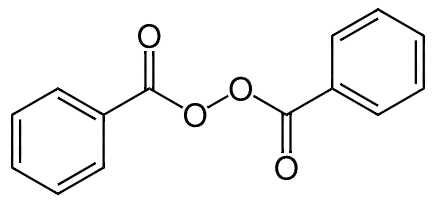
\includegraphics[scale=0.3]{00Figuras/POB-removebg-preview.png}
    \caption{a) peróxido de benzoilo}
    \label{POB}
\end{figure}

\begin{figure}[H]
    \centering
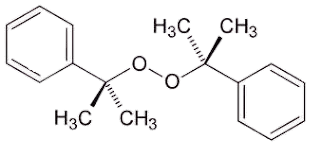
\includegraphics[scale=0.4]{00Figuras/PUC.png}
    \caption{b) peróxido de cumilo}
    \label{PUC}
\end{figure}


\section{Caracterización}



\textbf{Probetas:} 20 gramos de caucho molido de llanta y sobre eso se agrega 2\% del iniciador peróxido de benzoilo.

\textbf{Prensa:} Se utilizó la prensa hidráulica de 15 toneladas modelo MEGA KSC-15A, equipada con la bomba XX, para realizar la compresión de las probetas.

z

\section{Equipos}

Los equipos que se mencionan a continuación se utilizaron para caracterizar el material GTR original, así como las mezclas de GTR con agente desvulcanizante antes y después de la radiación con microondas. Esto permitió observar las características iniciales del material recibido, su composición, la cual influye en los resultados de la reacción, y evidenciar y comparar los posibles cambios ocurridos en los enlaces.


\subsection{Análisis termogravimétrico (TGA)}
Se utilizó un equipo TGA (Análisis Termogravimétrico) de Mettler Toledo para analizar los cambios de masa de la muestra en un rango de temperaturas de XX °C a XX °C, bajo una atmósfera inerte de XX a un flujo de XX mL/min y con una rampa de calentamiento de XX °C/min.

\begin{figure}[H]
    \centering
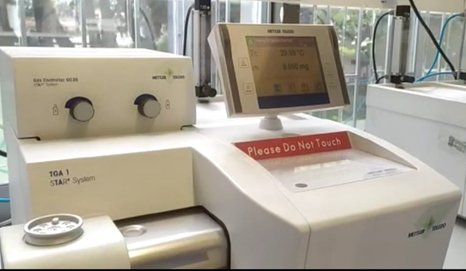
\includegraphics[scale=0.55]{00Figuras/TGA.png}
    \caption{\hl{Equipo TGA}}
    \label{TGA}
\end{figure}

\subsection{Calorimetría diferencial de barrido (DSC) }
Se utilizó un calorímetro diferencial de barrido (DSC) modelo \hl{HP DSC 1 STAR System} Mettler Toledo para analizar las propiedades térmicas de la muestra. Las mediciones se realizaron en un rango de temperaturas de xx °C a XX °C, bajo una atmósfera de XX a un flujo de XX mL/min. La muestra fue sometida a una tasa de calentamiento de XX °C/min. %Durante el análisis, se registraron las siguientes transiciones térmicas: \hl{explicar cuales se evidenciaron}

\begin{figure}[H]
    \centering
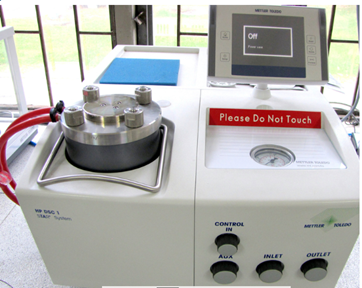
\includegraphics[scale=0.6]{00Figuras/DSC.png}
    \caption{\hl{Equipo DSC}}
    \label{DSC}
\end{figure}

\subsection{Espectroscopía infrarroja por transformada de Fourier (FTIR)}

La espectroscopía infrarroja por transformada de Fourier (FTIR) utilizando la técnica de XX se llevó a cabo con una resolución de XX \unit{cm^{-1}} y XX escaneos, en un rango de número de onda de XX a XX \unit{cm^{-1}}. Esta técnica se aplicó a las muestras que presentaron los mayores cambios en sus propiedades físicas durante el proceso de desvulcanización por microondas. Se anticipan modificaciones en los picos del espectro asociados a los enlaces S-S (565 \unit{cm^{-1}}) y C-S (XX \unit{cm^{-1}}).  

%Texto de prueba a ver qué tan bonito se ve.

%Segundo texto de prueba, se necesita probar mucho een esta vida.


\subsection{Reómetría}

Se utilizó un reómetro para medir las propiedades reológicas del caucho, modelo XX.

\subsection{Microondas-Magnetrón}

\section{Reacción}

\subsection{Microondas}

\begin{figure}[H]
    \centering
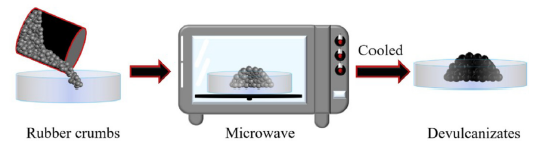
\includegraphics[scale=0.6]{00Figuras/microwave.png}
    \caption{\hl{TERMINAR DE MODIFICAR IMAGEN PROPIA DE ESTA}}
    \label{PUC}
\end{figure}

\end{multicols}


% \end{multicols}



\chapter{Info importante que NO va en el texto}

\begin{itemize}
    \item \hl{15 mg of each sample was heated from room temperature
to 560°C under nitrogen atmosphere at
heating rate of 10°C/min to monitor the weight loss
of oil and elastomers. At 560°C, the gas flow was
changed to oxygen atmosphere and the samples
were heated from 560 to 800°C in order to observe
the carbon black degradation. The experiments were performed
according to the following program: (A) Initial temperature
of 30°C; (B) Cooling: cooling rate of
30°C min–1 to –90°C; (C) Heating: heating rate of
30°C min–1 to 250°C. The results reported in this
work correspond to the heating runs. All DSC curves
were normalized according to the sample mass.}

\item \hl{The soluble (sol) and insoluble (gel) fractions of
each sample, after the devulcanization process, were
determined by Soxhlet extraction, by using toluene
about 4 g of GTR was immersed in toluene for
6 h at 80°C. After extraction, the samples were
dried for 24 h at 80°C to remove the solvent and
their masses were measured}

\item In another study,
chemical and mechano-chemical methods were used by Rooj et al. [51] for devulcanizing natural
rubber (NR) utilizing benzoyl peroxide as a devulcanization aid. As the outcomes revealed, sulfur
crosslink happened selectively at the optimum temperature and optimum time of 80 °C and 6 h,
respectively. 

\item sol-gel measurements
acetone was used as the extraction solvent for a minimum time of 12 h before performing
the swelling test. Then, the samples were dehumidified in an oven until reaching a constant weight A small amount of sample was immersed in toluene for 3 days at room temperature.
Afterward, it was placed in an oven at 80 \unit{\degreeCelsius} C until reaching a constant weight


\item Crosslink density measurements
Crosslink density of the gel part of the virgin sample and samples devulcanized by DSO and
TMTD was measured by the swelling test utilizing toluene solvent. The crosslinking density was
determined using the Fluorine-Renner equation (Equation 2), and the interaction parameter ()
assumed to be 0.45 for the toluene-rubber system

\item At 80 C, benzoyl peroxide undergoes free
radical chain scission, which produces highly unstable
benzoyl radicals. Due to its instability, it spontaneously
reacts with the sulfur present in the cured rubber. It is well
known that the bond energy of S–S (227 kJ/mol) and C–S
bonds (273 kcal/mol) is lower than that of the C–C bond
(348 kJ/mol)

The bond energy of different chemical bonds is as
follows: 348 kJ/mol for C–C, 621 kJ/mol for C=C, 416 kJ/
mol for C–H, 273 kJ/mol for C–S, 227 kJ/mol for S–S and
378 kJ/mol for C–C= in CH3-CH=CH2 compound

\end{itemize}

\subsection{Posibles normas a leer}

Reologia: ASTM D-2084-11
SWELLING TEST: ASTM D6814-02
Mooney viscosimeter ASTM D1646.
Free sulfur ASTM D297-72A
Mechanical properties ASTM D 412
Durometer ASTM D 2240 


\chapter{Resultados}

\begin{multicols}{2}

\subsection{Caracterización del GTR}

Para caracterizar el material GTR original, se realizaron los siguientes análisis:  
\begin{itemize}
    \item TGA  
    \item DSC  
    \item FTIR  
    \item Reometría  
\end{itemize}

\subsection{Desvulcanización}

El efecto de la radiación por microondas sobre el material se evaluó sometiéndolo a diferentes tiempos de irradiación: x, x, x, x y x \hl{segundos}, y variando el porcentaje de agente desvulcanizante. Durante el proceso, se registraron los cambios físicos observados, como el color del humo (en caso de generarse), la fluidez del material, la descomposición, y se midió la temperatura dentro del equipo. % Cabe destacar que algunas muestras podrían destruirse o incendiarse durante el experimento.

\subsection{Caracterización del GTR con agentes desvulcanizantes}

\subsubsection{Antes de la radiación por microondas}

Las mezclas de GTR con agentes desvulcanizantes se caracterizaron mediante:  
\begin{itemize}
    \item TGA  
    \item DSC  
    \item FTIR  
    \item Reometría  
\end{itemize}

\subsubsection{Después de la radiación por microondas}

Posterior a la radiación, las muestras se caracterizaron utilizando las mismas técnicas:  
\begin{itemize}
    \item TGA  
    \item DSC  
    \item FTIR  
    \item Reometría  
\end{itemize}

\end{multicols}

\subsection{Resultados Obtenidos}

\subsection{Resultados esperados \hl{acorde a la literatura}}

\begin{enumerate}
    \item parcial devulcanization for disulfide (-S2-) and poly-sulfide (-SX-) pero dificultad en romper enlaces C-S (monosulfidicos) debido a la energia proveida por las ondas microondas.
  
    %a temperatura de reacción, 

    \item Ojo las propiedades del cauco se disminuyen debido a la escisión mediante microondas!.
    Al aumentar el tiempo de reacción y la cantidad de agentes de desvulcanización, se observaría una disminución en la densidad de enlaces cruzados y un aumento en el porcentaje de desvulcanización. \hl{the higher the sol fraction of the samples
devulcanized by devulcanizing agent, the higher the devulcanization percentage}



\item by enhancing the \hl{enhancing devulcanazing agent content up to 5 phr, the volume fraction and crosslink density of rubber decrease while the sol fraction and devulcanization porcentaje increase}

\item FTIR
Disminucion en pico S-S (556), que no haya cambios en picos C-C (Stretching vibrations), lo que indica que (main polymer bonds have not been destroyed) como no hay grandes cambios en el espectro --> demonstrating that the breakdown of the main chains does not happen in
the polymer \cite{Zhang2024AnDevulcanization}.

\item temperature of 150 C and a pressure of 5 MPa for 8 min
in an electrically heated press

\end{enumerate}
\chapter{Resultados}





\chapter{Conclusiones}
\chapter{Recomendaciones}

%Inicio del apéndice o anexos
\begin{appendix}
\chapter{Apéndice 1}%
\end{appendix}

%Permite visualizar la bibliografía en la tabla de contenido
%Cambie el nombre a Bibliografía o Literatura Citada en la siguiente línea de ser preciso
\addcontentsline{toc}{chapter}{Referencias Bibliográficas} 

\let\OLDthebibliography=\thebibliography
\def\thebibliography#1{\OLDthebibliography{#1}}
{\scriptsize
\pagestyle{plain}
% Nombre del documento donde se almacenan las referencias
\bibliography{Referencias}
\nocite{*}
% Inserta un página adicional al final en blanco 
%\cleardoublepage
% Para NO insertar una página adicional al final usar \clearpage
\clearpage
}}

\end{document}